\documentclass[11pt,a4paper]{article}
\usepackage[utf8]{inputenc}
\usepackage[margin=1in]{geometry}
\usepackage{amsmath, amssymb}
\usepackage{booktabs}
\usepackage{tikz}
\usetikzlibrary{arrows.meta, positioning, fit}
\usepackage{titlesec}
\titlespacing*{\section}{0pt}{1.4ex plus .2ex minus .2ex}{0.8ex plus .1ex}

\title{\texttt{IKCompiler.calc\_angle\_config()}}
\author{}
\date{}

\begin{document}
\sloppy

\maketitle
\vspace{-3.5em}

\begin{center}
\resizebox{!}{0.62\textheight}{%
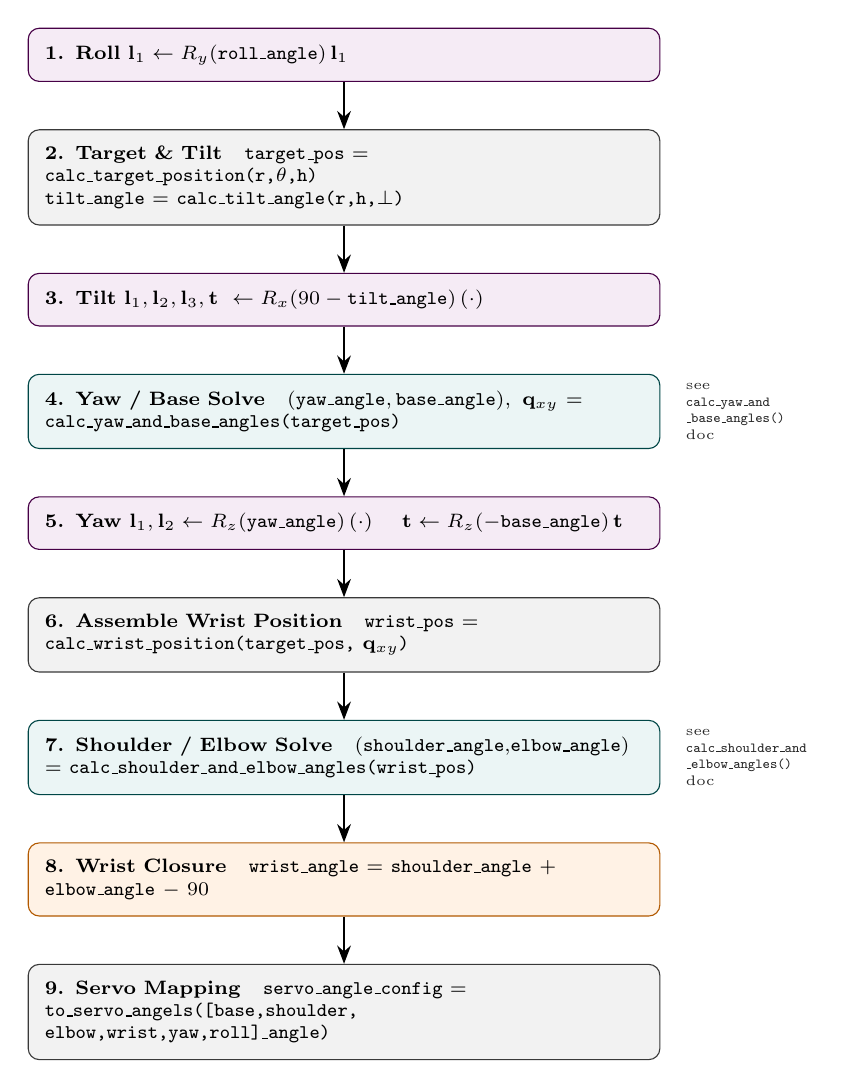
\begin{tikzpicture}[
    node distance=6mm and 0mm,
    box/.style={draw, rounded corners, align=left, text width=7.6cm, font=\scriptsize, inner sep=6pt},
    vec/.style={box, fill=violet!8, draw=violet!55!black},
    solve/.style={box, fill=teal!8, draw=teal!55!black},
    asm/.style={box, fill=gray!10, draw=gray!45!black},
    der/.style={box, fill=orange!10, draw=orange!70!black},
    tag/.style={font=\tiny, text=gray!30!black, align=left},
    >=Stealth
]

\node[vec] (b1) {\textbf{1. Roll} $\mathbf l_1 \gets R_y(\texttt{roll\_angle})\,\mathbf l_1$};

\node[asm, below=of b1] (b2) {\textbf{2. Target \& Tilt}\quad
\texttt{target\_pos} = \texttt{calc\_target\_position(r,}$\theta$\texttt{,h)} \\
\texttt{tilt\_angle} = \texttt{calc\_tilt\_angle(r,h,}$\perp$\texttt{)}};

\node[vec, below=of b2] (b3) {\textbf{3. Tilt} $\mathbf l_1,\mathbf l_2,\mathbf l_3,\mathbf t
\ \gets R_x(90-\texttt{tilt\_angle})\,(\cdot)$};

\node[solve, below=of b3] (b4) {\textbf{4. Yaw / Base Solve}\quad
$(\texttt{yaw\_angle},\texttt{base\_angle}),\ \mathbf q_{xy}$
= \texttt{calc\_yaw\_and\_base\_angles(target\_pos)}};
\node[tag, right=2mm of b4] {see\\\texttt{calc\_yaw\_and}\\\texttt{\_base\_angles()}\\doc};

\node[vec, below=of b4] (b5) {\textbf{5. Yaw} $\mathbf l_1,\mathbf l_2 \gets R_z(\texttt{yaw\_angle})\,(\cdot)$
\quad $\mathbf t \gets R_z(-\texttt{base\_angle})\,\mathbf t$};

\node[asm, below=of b5] (b6) {\textbf{6. Assemble Wrist Position}\quad
\texttt{wrist\_pos} = \texttt{calc\_wrist\_position(target\_pos,} $\mathbf q_{xy}$\texttt{)}};

\node[solve, below=of b6] (b7) {\textbf{7. Shoulder / Elbow Solve}\quad
(\texttt{shoulder\_angle},\texttt{elbow\_angle}) =
\texttt{calc\_shoulder\_and\_elbow\_angles(wrist\_pos)}};
\node[tag, right=2mm of b7] {see\\\texttt{calc\_shoulder\_and}\\\texttt{\_elbow\_angles()}\\doc};

\node[der, below=of b7] (b8) {\textbf{8. Wrist Closure}\quad
\texttt{wrist\_angle} = \texttt{shoulder\_angle} + \texttt{elbow\_angle} $-\ 90$};

\node[asm, below=of b8] (b9) {\textbf{9. Servo Mapping}\quad
\texttt{servo\_angle\_config} = \texttt{to\_servo\_angels([base,shoulder,}\\
\texttt{elbow,wrist,yaw,roll]\_angle)}};

\foreach \x/\y in {b1/b2, b2/b3, b3/b4, b4/b5, b5/b6, b6/b7, b7/b8, b8/b9}
  \draw[->, thick] (\x) -- (\y);

\end{tikzpicture}}
\end{center}

\noindent
\textcolor{violet!55!black}{\textbf{Violet}}: rotates one or more of the four translation
vectors $\mathbf l_1,\mathbf l_2,\mathbf l_3,\mathbf t$ in place.
\textcolor{teal!55!black}{\textbf{Teal}}: delegates to an already-documented solve.
\textbf{Gray}: pure assembly/bookkeeping. \textcolor{orange!70!black}{\textbf{Orange}}: a
closed-form step derived here.

\section{Setup}

\begin{align*}
\mathbf l_1 = (0,0,L_1), \quad
\mathbf l_2 = (L_2,0,0), \quad
\mathbf l_3 = (0,0,L_3), \quad
\mathbf t = (0,0,\texttt{wrist\_arm\_length})
\end{align*}
are \texttt{self} attributes -- they persist and are mutated \emph{in place} across the whole
method. \texttt{roll\_angle} and
\texttt{wrist\_perpendicular\_2\_ground} ($\perp$ above) are free inputs: \texttt{roll\_angle}
is never solved for, only used to orient $\mathbf l_1$ and passed straight through to the
output.

\section{Transform Bookkeeping}

Steps 1, 3, 5 apply a different subset of \{roll, tilt, yaw/base\} to each vector:

\begin{center}
\begin{tabular}{@{}lccc@{}}
\toprule
vector & roll ($y$) & tilt ($x$, $90-\texttt{tilt\_angle}$) & yaw/base ($z$) \\
\midrule
$\mathbf l_1$ & \checkmark & \checkmark & \checkmark\ \texttt{yaw\_angle} \\
$\mathbf l_2$ & -- & \checkmark & \checkmark\ \texttt{yaw\_angle} \\
$\mathbf l_3$ & -- & \checkmark & -- \\
$\mathbf t$   & -- & \checkmark & \checkmark\ $-\texttt{base\_angle}$ \\
\bottomrule
\end{tabular}
\end{center}

This asymmetry looks worse than it is. A $z$-axis rotation leaves the $z$ component fixed:
\begin{equation}
R_z(\theta) = \begin{bmatrix}\cos\theta & -\sin\theta & 0\\ \sin\theta & \cos\theta & 0\\
0 & 0 & 1\end{bmatrix}
\qquad\Longrightarrow\qquad \big(R_z(\theta)\,\mathbf v\big)_z = v_z
\end{equation}
and \texttt{calc\_wrist\_position} (\S\ref{sec:assemble}) only ever reads
$(\mathbf l_1+\mathbf l_2+\mathbf l_3)_z$ -- never their $x,y$. So step 5's yaw rotation of
$\mathbf l_1,\mathbf l_2$, and $\mathbf l_3$ never receiving one, make \emph{no difference to
this call's return value}: the $z$-sum is identical either way. They do still overwrite
\texttt{self.l1\_translation\_vec} / \texttt{self.l2\_translation\_vec} with new $x,y$ --
state that only matters if something later reads those vectors' full 3D value (nothing
currently does). $\mathbf t$ is the one vector whose full vector (not just $z$) is used, so its
yaw/base rotation in step 5 is the one that actually matters for the result.

\section{Assembling the Wrist Position}
\label{sec:assemble}

\begin{align}
\texttt{yaw\_position}_z &= \big(\texttt{target\_pos} + \mathbf l_1+\mathbf l_2+\mathbf l_3\big)_z \\
\texttt{yaw\_position} &= (q_x,\, q_y,\, \texttt{yaw\_position}_z) \\
\texttt{wrist\_pos} &= \texttt{yaw\_position} + \mathbf t
\end{align}
$q_x,q_y$ come from the circle-tangent solve in \texttt{calc\_yaw\_and\_base\_angles} -- this
step is pure vector addition, no new geometry is solved here.

\section{Wrist Closure}

Let $\phi$ be the world elevation (angle from horizontal) of segment $E\mathbf w$ -- the
elbow-to-wrist link, continuing the notation of the shoulder/elbow doc. At full extension
($\texttt{elbow\_angle}=180^\circ$) $\phi$ equals \texttt{shoulder\_angle}; bending away from
that by $(180^\circ - \texttt{elbow\_angle})$ gives, in general,
\begin{equation}
\phi = \texttt{shoulder\_angle} + \texttt{elbow\_angle} - 180^\circ
\end{equation}
\texttt{wrist\_angle} follows the same ``$90^\circ$ = neutral'' servo convention used
throughout (\texttt{calc\_tilt\_angle}, \texttt{to\_servo\_angels}):
\begin{equation}
\raisebox{-0.5\height}{\tikz \node[draw=orange!70!black, line width=1.4pt, rounded corners=3pt,
fill=orange!8, inner sep=12pt]
{\Large $\displaystyle \texttt{wrist\_angle} = \phi + 90^\circ =
\texttt{shoulder\_angle} + \texttt{elbow\_angle} - 90^\circ$};}
\end{equation}
This assumes the shoulder/elbow solve reproduces the same orientation the earlier vector
rotations (steps 1--5) already committed $\mathbf t$ to -- i.e.\ the two halves of the method
are only consistent because \texttt{tilt\_angle} and the shoulder/elbow triangle are both
driven by the same \texttt{target\_pos}.

\section{Notation $\leftrightarrow$ Code}

\begin{center}
\begin{tabular}{@{}ll@{}}
\toprule
Symbol & Variable \\
\midrule
$\mathbf l_1,\mathbf l_2,\mathbf l_3$ & \texttt{l1\_translation\_vec}, \texttt{l2\_translation\_vec}, \texttt{l3\_translation\_vec} \\
$\mathbf t$ & \texttt{tilt\_translation\_vec} \\
$\mathbf q_{xy}$ & \texttt{yaw\_pos\_xy} \\
$\phi$ & (elevation of segment $E\mathbf w$, not itself a variable) \\
\bottomrule
\end{tabular}
\end{center}

\end{document}
